\documentclass[11pt,a4paper]{article}
\usepackage[utf8]{inputenc}
\usepackage[spanish]{babel}
\usepackage{amsmath}
\usepackage{amsfonts}
\usepackage{amssymb}
\usepackage{graphicx}
\usepackage{geometry}
\usepackage{xcolor}
\usepackage{hyperref}
\usepackage{float}

\geometry{margin=2.5cm}

\title{
    \vspace{-2cm}
    \textbf{\Large Universidad Externado de Colombia} \\
    \large Pregrado en Ciencia de Datos \\
    \vspace{0.5cm}
    \textbf{\huge Taller Integrado de Regresión Bayesiana} \\
    \large Caso Uber y Venta de Boletas Movistar Arena \\
    \textit{Estadística Bayesiana}
}

\author{
    \textbf{Equipo de Trabajo:} \\
    Julian Camilo, Julián Duarte, Tomás Rincón \\
    \textit{Facultad de Ciencia de Datos}
}

\date{\today}

\begin{document}

\maketitle

\section*{Introducción}
Imagina una noche de viernes en Bogotá: miles de personas salen de un concierto en el \textbf{Movistar Arena} y todos comparten la misma pregunta: ¿Cómo volver a casa? Este taller explora ese momento, utilizando la estadística bayesiana para entender el comportamiento de los usuarios de \textbf{Uber Pool} y la logística alrededor del evento. Nuestro objetivo es transformar la incertidumbre de una ciudad en movimiento en decisiones estratégicas informadas, contando la historia de cómo los datos se convierten en soluciones.

\section{Parte I: Regresión Lineal Bayesiana}
El propósito de esta parte es analizar mediante regresión lineal bayesiana relaciones relevantes en el experimento de Uber Pool para evaluar la viabilidad operativa del servicio en Bogotá.

\subsection{Desarrollo del modelo y Selección Inicial de Variables}
Para comenzar, planteamos una \textbf{hipótesis inicial} de las variables que \textit{creemos} que serán útiles para nuestro modelo, basándonos puramente en la lógica del negocio. Es importante aclarar que esta es solo una selección preliminar (hipótesis) que, más adelante, será sometida a validación matemática.

Bajo esta premisa lógica, el modelo lineal bayesiano propuesto tendría la forma general:
\bigskip
\begin{center}
    $y_i = \beta_0 + \beta_1 X_{1i} + \beta_2 X_{2i} + \dots + \beta_k X_{ki} + \epsilon_i$,  $\epsilon_i \sim N(0, \sigma^2)$
\end{center}
\bigskip

donde nuestras variables candidatas iniciales son:
\begin{itemize}
    \item $y_i$ (\textit{rider\_cancellations}):
    \begin{itemize}
        \item \textbf{Descripción:} Cantidad de cancelaciones por parte del pasajero en cada periodo.
        \item \textbf{Justificación:} Elegimos esta variable porque es el indicador más directo de la \textbf{fricción del usuario}. Mientras que los ingresos dependen de factores externos como tarifas dinámicas, las cancelaciones capturan el punto de quiebre de la paciencia del cliente bogotano frente a la espera.
    \end{itemize}
    \item $X_{1i}$ (\textit{total\_matches}) y $X_{2i}$ (\textit{trips\_pool}):
    \begin{itemize}
        \item \textbf{Descripción:} Volumen de emparejamientos y viajes completados.
        \item \textbf{Justificación:} Actúan como variables de \textbf{control estructural}. Capturan la escala de actividad en el periodo; al incluirlas, aseguramos que el efecto del tratamiento que encontremos no sea simplemente un subproducto de tener "más gente en la calle", sino un efecto puro de la política de espera.
    \end{itemize}
    \item $X_{3i}$ (\textit{treat}):
    \begin{itemize}
        \item \textbf{Descripción:} Variable binaria (1 si el tiempo de espera configurado es 5 min, 0 si es 2 min).
        \item \textbf{Justificación:} Es nuestro \textbf{predictor experimental}. Nos permite cuantificar exactamente cuánto aumenta el riesgo de cancelación al estirar el umbral de espera del usuario.
    \end{itemize}
    \item $X_{4i}$ (\textit{commute}):
    \begin{itemize}
        \item \textbf{Descripción:} Variable binaria para horas pico (7-9:40am o 3-5:40pm).
        \item \textbf{Justificación:} Necesaria para aislar el efecto de la congestión y el estrés urbano del horario bogotano, que es un disparador natural de impaciencia.
    \end{itemize}
    \item $\sigma^2$ (Varianza del Error):
    \begin{itemize}
        \item \textbf{Descripción:} Un número positivo que mide el margen de error.
        \item \textbf{Justificación:} Representa todo lo que nuestro modelo no alcanza a explicar, ya que el comportamiento humano nunca es 100\% predecible.
    \end{itemize}
\end{itemize}

\subsubsection*{Paso 1: Análisis Exploratorio de Datos (EDA)}
Antes de construir el modelo bayesiano, realizamos un Análisis Exploratorio de Datos (EDA) guiado por visualizaciones en Python para entender el comportamiento real del servicio en Bogotá.

Primero, analizamos nuestra variable objetivo (\textit{trips\_pool}). Encontramos que, en promedio, se completan 1,408 viajes compartidos por periodo (donde cada periodo representa una ventana de tiempo de 160 minutos, lo que equivale a 9 segmentos por día), con una desviación estándar de $\approx 257$ viajes. Este es el comportamiento base que nuestros predictores deberán intentar explicar.

A continuación, visualizamos cómo nuestras covariables afectan la cantidad de viajes:

\begin{figure}[H]
    \centering
    \begin{minipage}{0.48\textwidth}
        \centering
        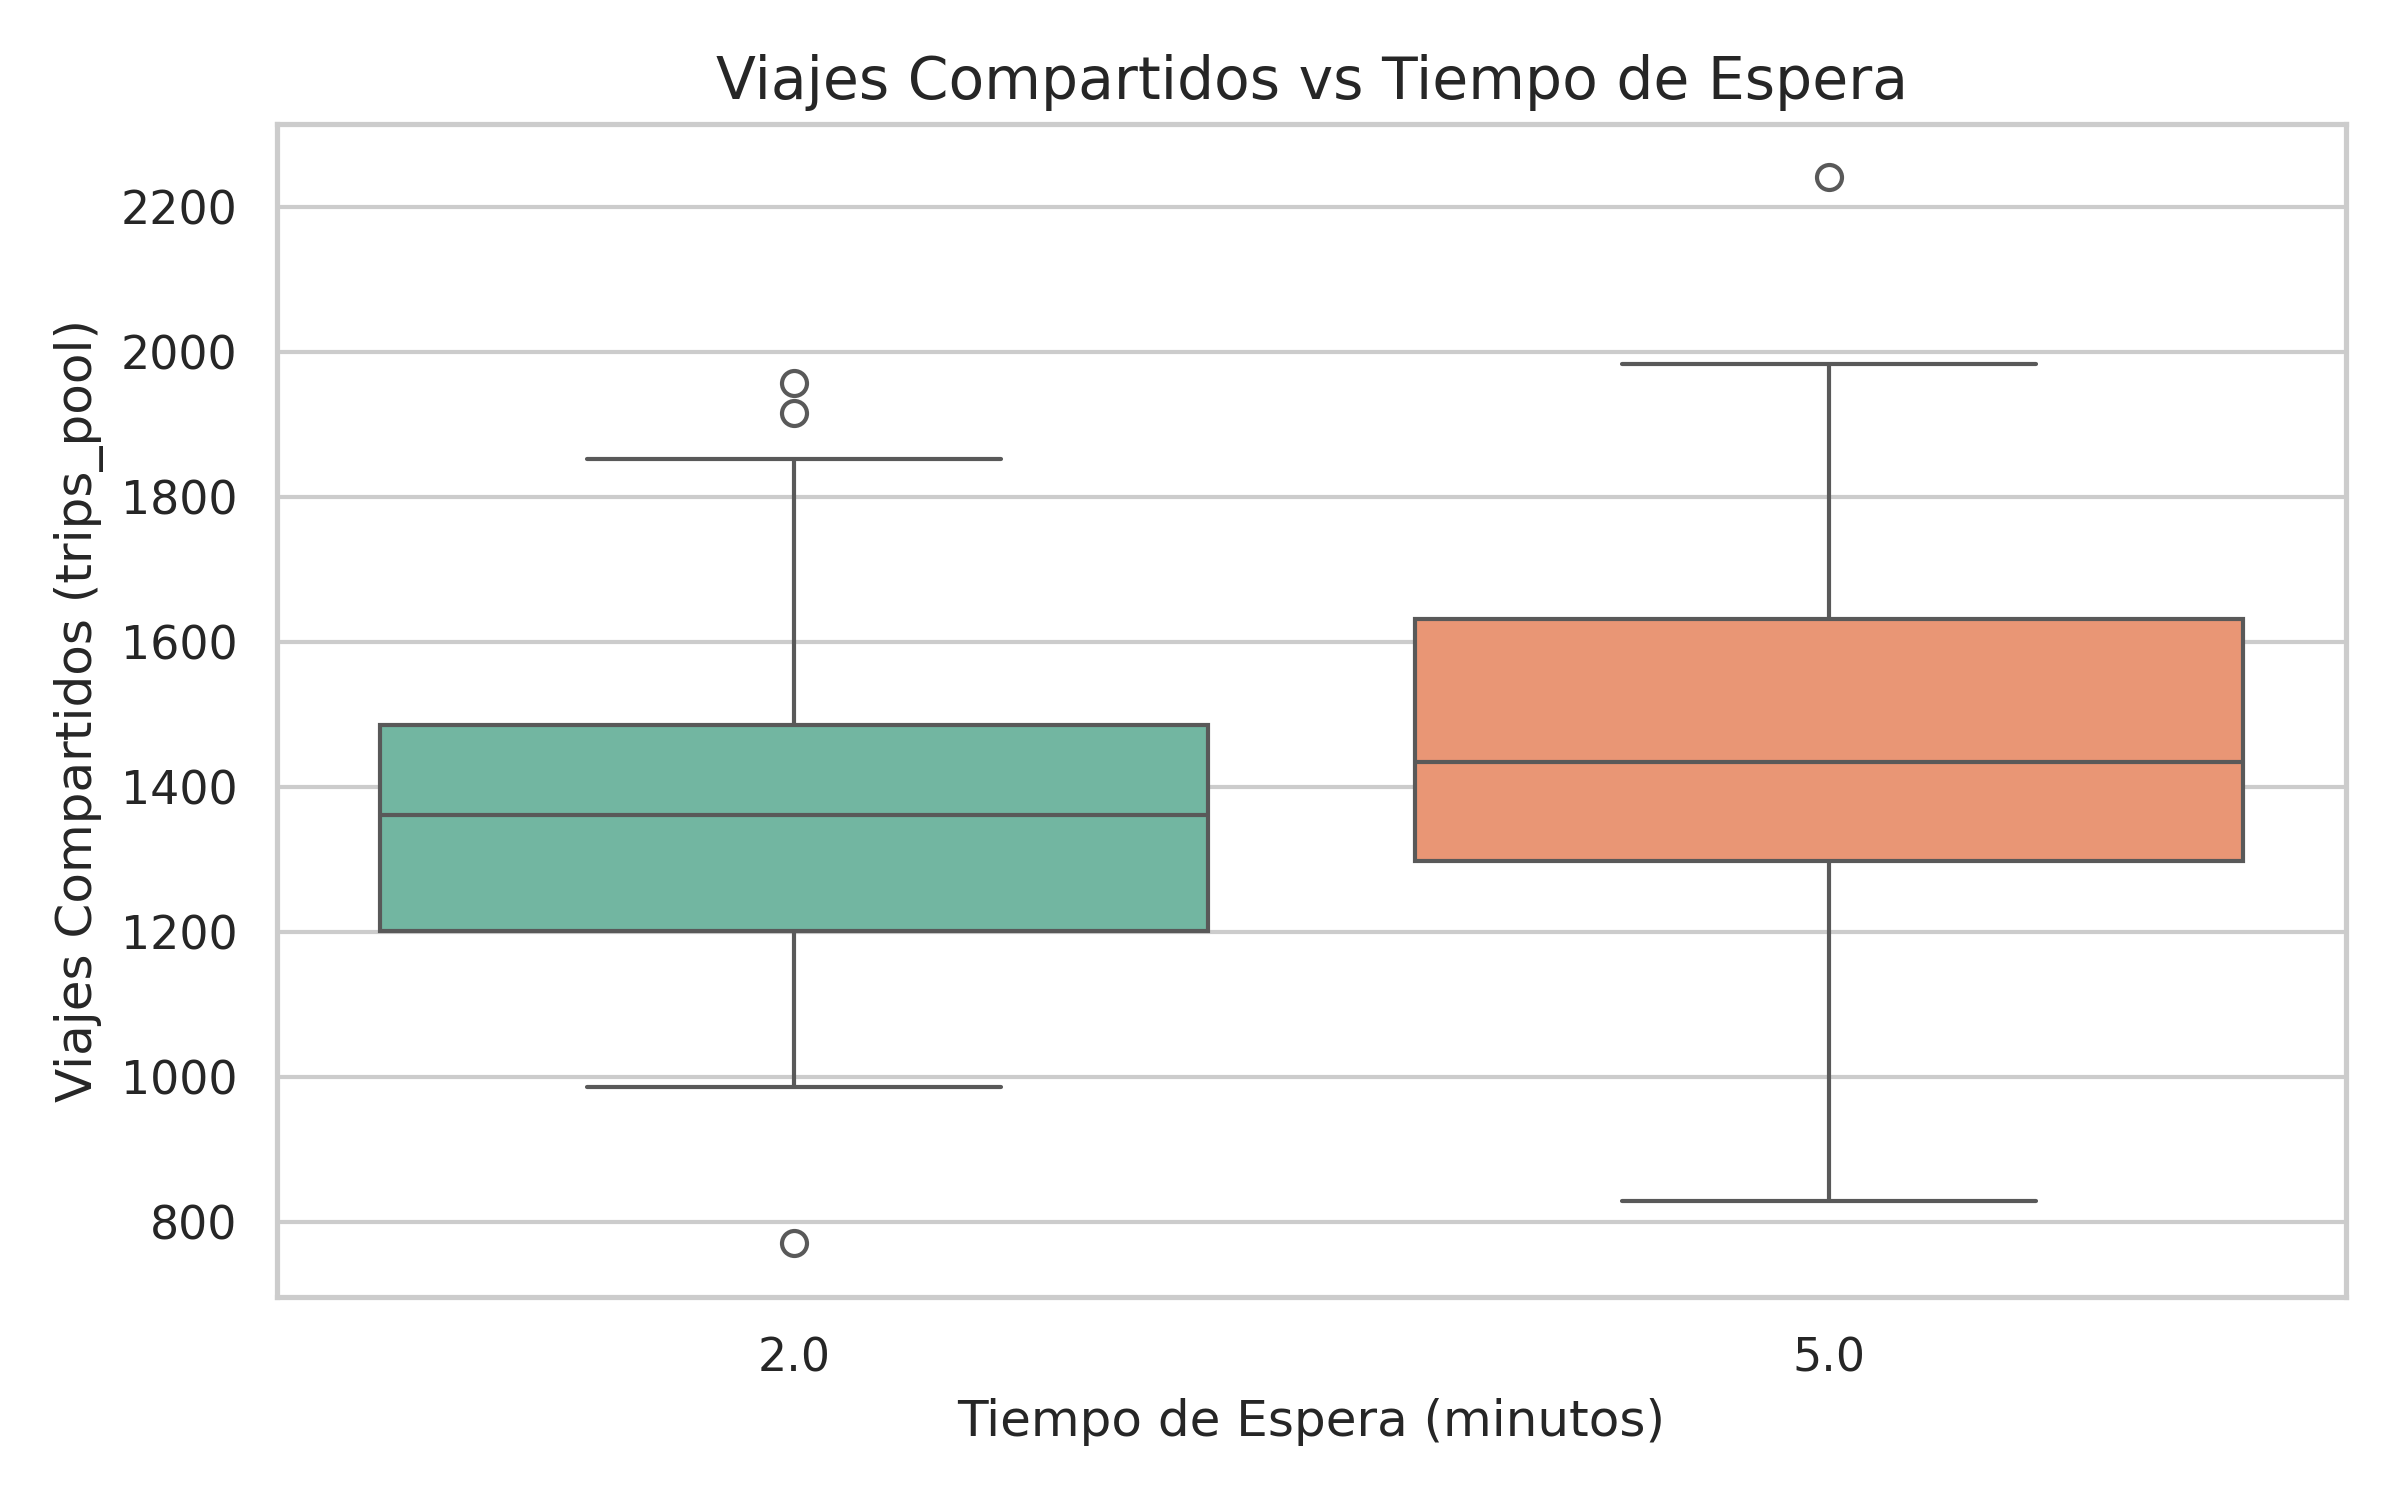
\includegraphics[width=\linewidth]{img/uber/eda_wait_time.png}
        \caption{Viajes según el tiempo de espera}
    \end{minipage}\hfill
    \begin{minipage}{0.48\textwidth}
        \centering
        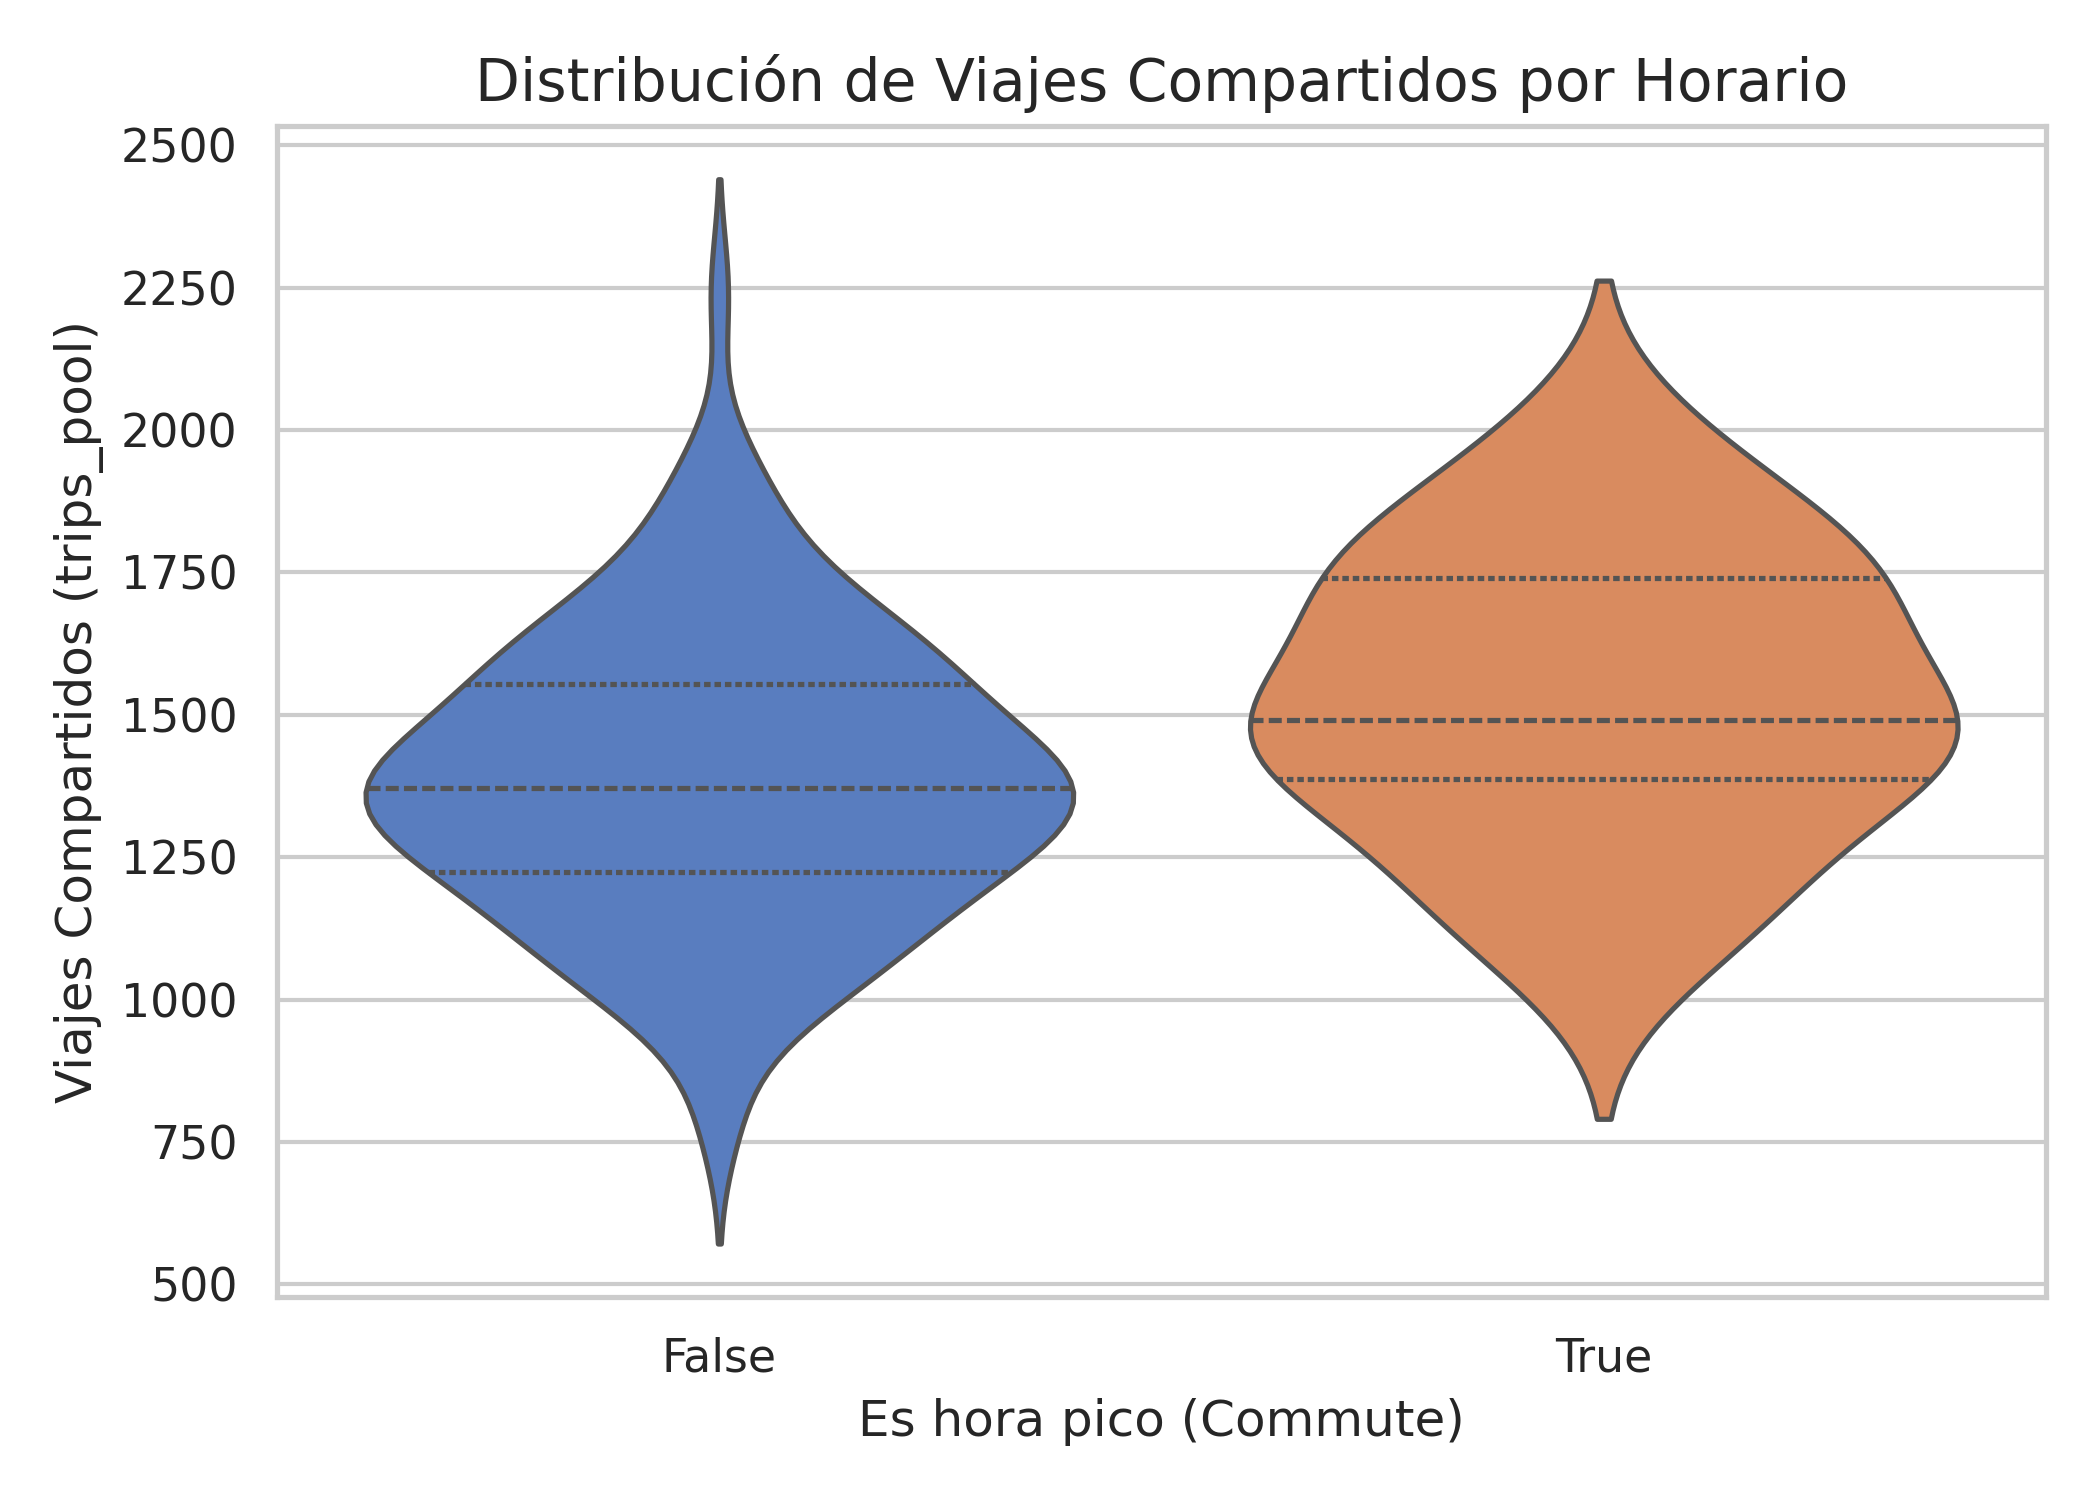
\includegraphics[width=\linewidth]{img/uber/eda_commute.png}
        \caption{Viajes según horario (Hora Pico vs Normal)}
    \end{minipage}
\end{figure}

Al observar estas gráficas, confirmamos dos puntos muy importantes para nuestro modelo:
\begin{itemize}
    \item \textbf{Efecto del tiempo de espera:} El primer gráfico nos muestra algo sumamente interesante (y contraintuitivo): al pasar el tiempo de espera estimado de 2 a 5 minutos, la cantidad media de viajes no sufre una caída drástica, sino que se mantiene sorprendentemente estable (o incluso con un levísimo aumento). Esto sugiere que la demanda del servicio es inelástica frente a una demora de 3 minutos extra.
    \item \textbf{Efecto de la hora pico:} En el segundo gráfico, al comparar horarios normales (0) frente a las horas pico (1), notamos que la demanda tiene un comportamiento muy similar en ambas franjas, aunque con picos ligeramente superiores durante el \textit{commute}. Seguiremos utilizando la variable para validar esto estadísticamente, pero de entrada la diferencia visual no es extrema.
\end{itemize}

\subsubsection*{Paso 2: Validación y Matriz de Correlación}
Después de confirmar el impacto individual de cada variable, debíamos asegurarnos de que no hubiera problemas de multicolinealidad. Si incluimos dos variables que miden exactamente lo mismo, el modelo no podrá identificar cuál de las dos es la causante real de un cambio y el cálculo matemático fallará. Para revisar esto, generamos una matriz de correlación de Pearson:

\begin{figure}[H]
    \centering
    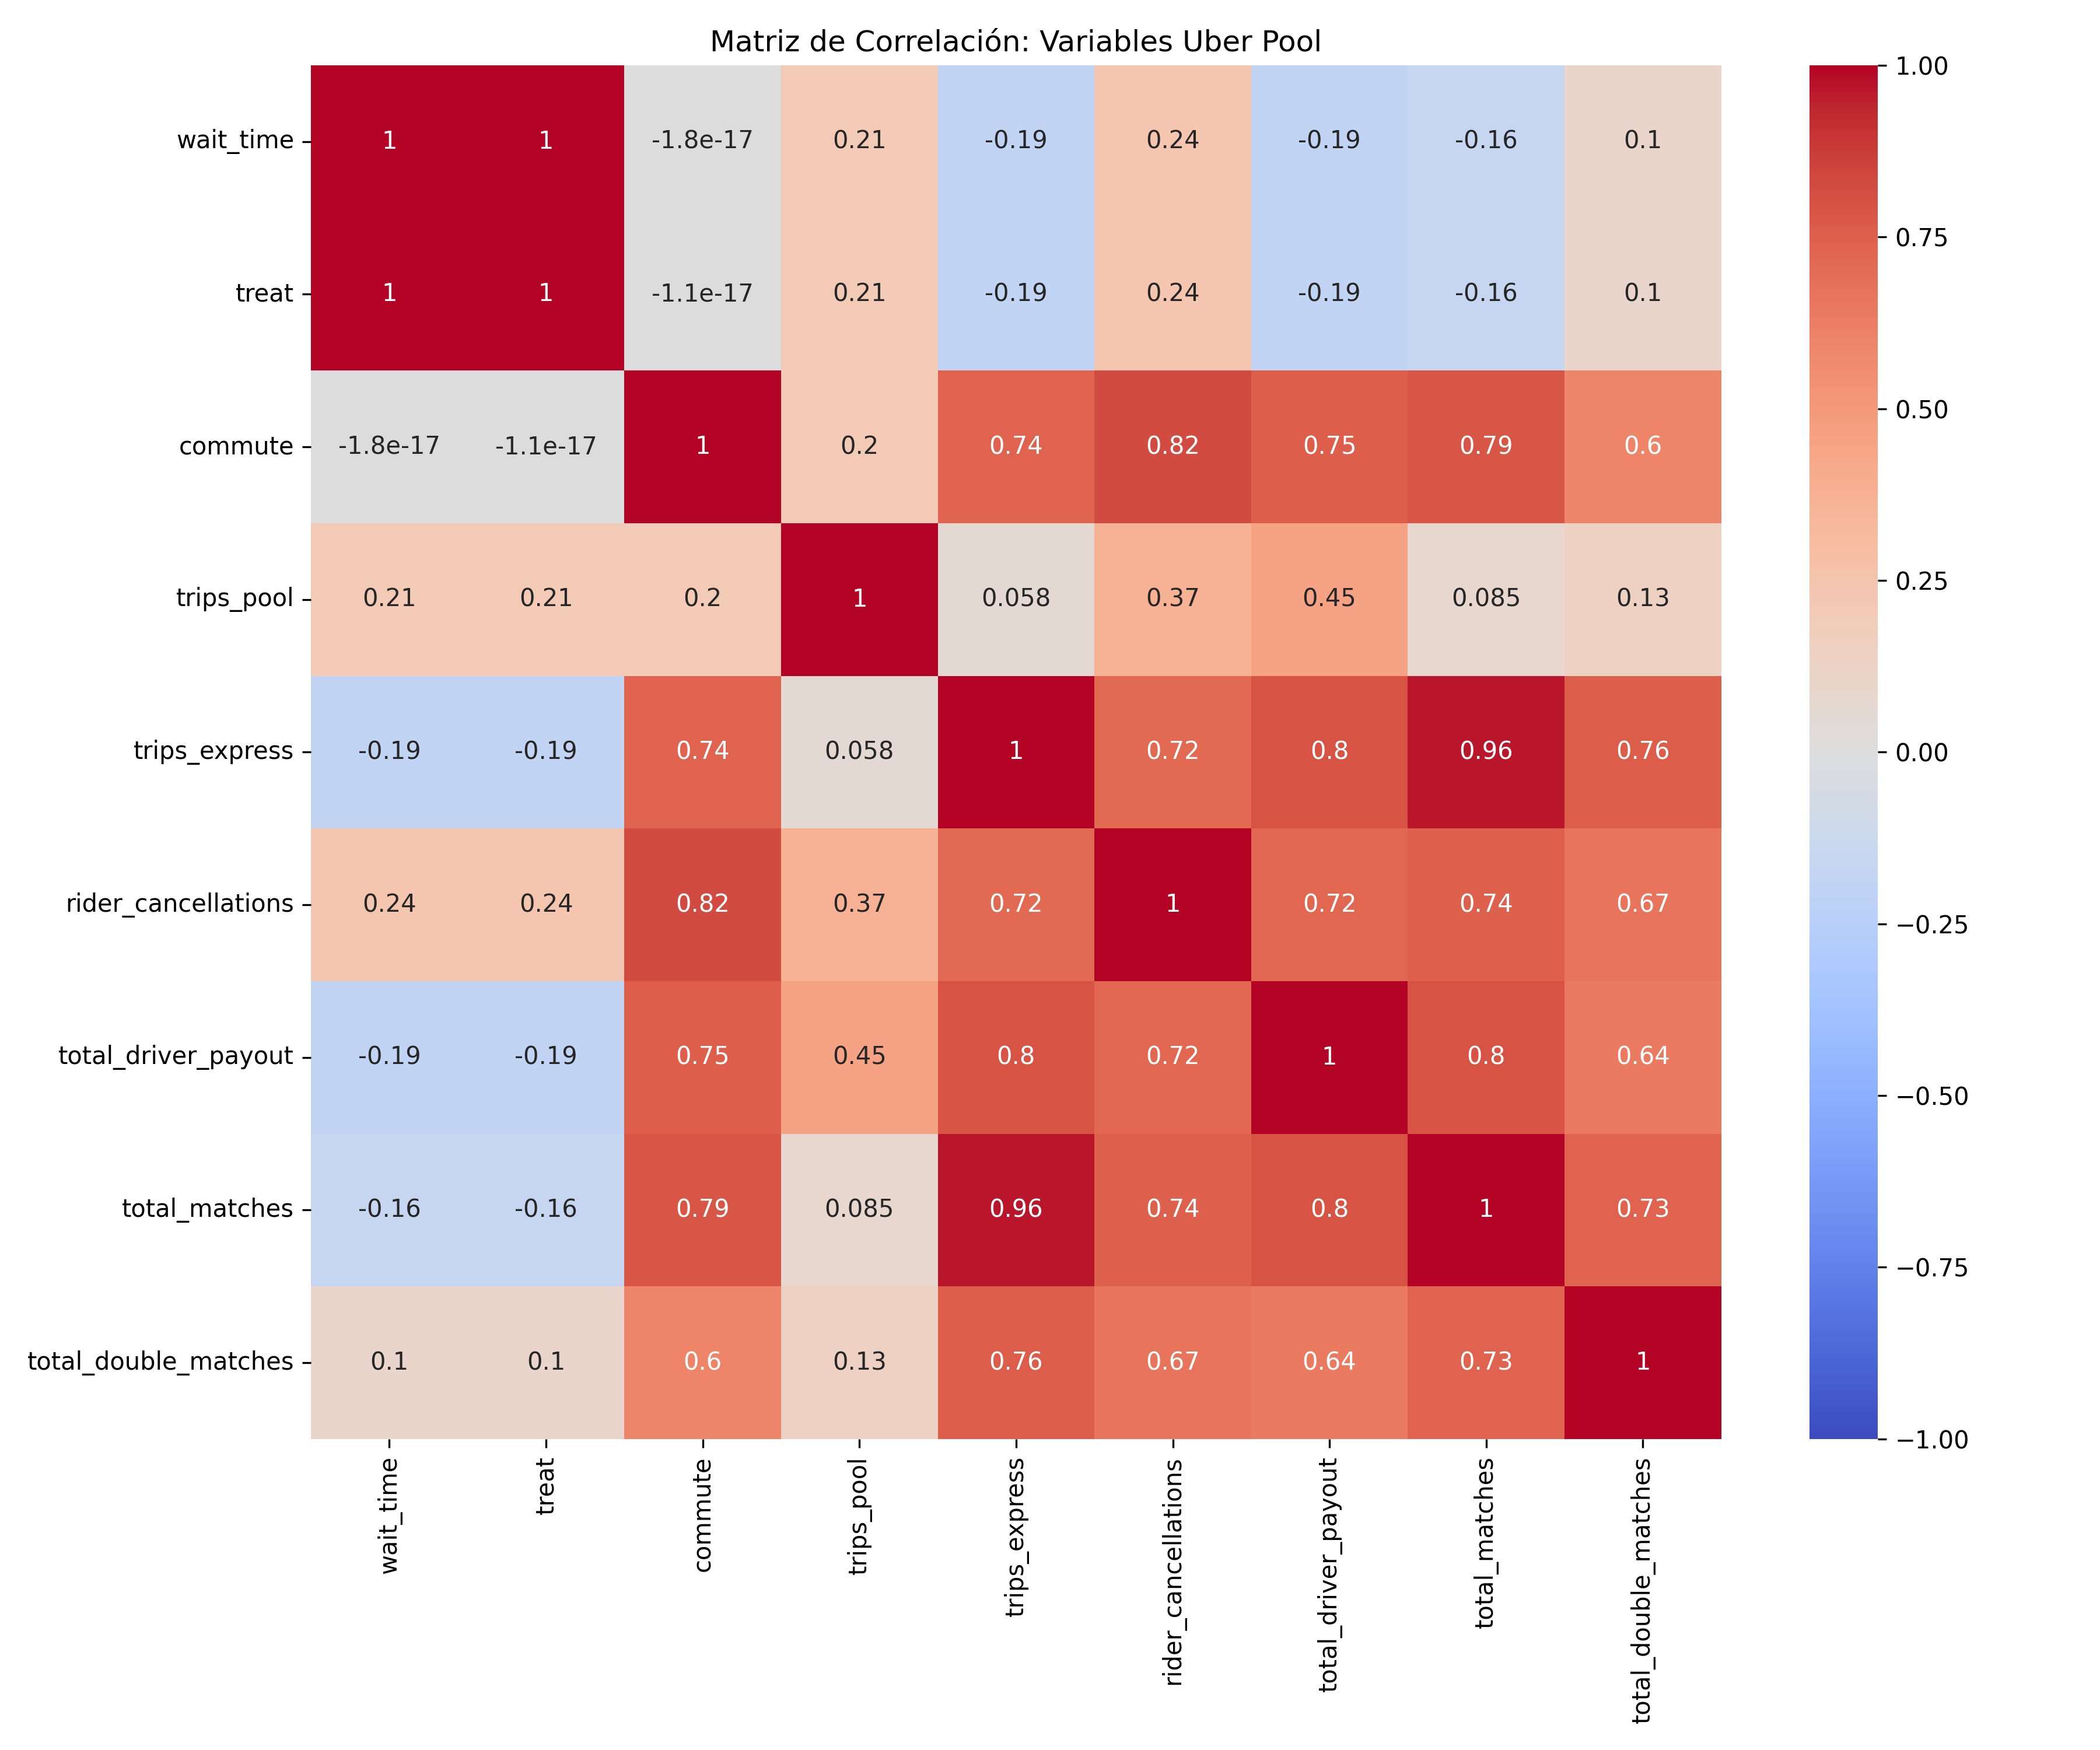
\includegraphics[width=0.55\textwidth]{img/uber/uber_correlation.png}
    \caption{Matriz de Correlación: Evaluando redundancias entre predictores}
    \label{fig:corr_uber}
\end{figure}

Al ver los resultados en esta matriz, nos llevamos una sorpresa clave: hay una \textbf{correlación perfecta (1.0)} entre la variable \textit{treat} (que simplemente dice si el usuario era parte del experimento o no) y la variable \textit{wait\_time} (el tiempo de espera). ¿Qué significa esto en la vida práctica? Nos confirma que "aplicar el tratamiento" se basó única y exclusivamente en subir los tiempos de espera a esos usuarios. 

Como ambas variables miden exactamente la misma información, si las ponemos juntas, nuestro modelo matemático va a colapsar porque no sabrá a cuál de las dos atribuirle el impacto en los viajes. Por esta gran razón estadística, \textbf{decidimos sacar la variable \textit{treat}}. Nos quedaremos únicamente con \textit{wait\_time}, dado que medir el problema en "minutos" es mucho más lógico y fácil de explicar que un "sí o no".

\subsubsection*{Conclusión: Selección Definitiva de Variables}
Tras revisar la información y analizar las correlaciones entre variables, la conclusión es que nuestra lista inicial debía cambiar. A continuación explicamos, de forma muy sencilla, con qué partes de la base de datos nos quedamos y cuáles descartamos:

\textbf{Variables Conservadas:}
\begin{itemize}
    \item \textbf{\textit{trips\_pool}:} Se queda porque es lo que queremos adivinar (viajes totales de Uber Pool).
    \item \textbf{\textit{wait\_time}:} Se queda porque es el tiempo de espera en minutos que Uber cambió a propósito. Usar los minutos nos permite explicar resultados de forma muy natural.
    \item \textbf{\textit{commute}:} Se queda porque necesitamos separar la alta demanda de la hora pico frente a un horario normal.
\end{itemize}

\textbf{Variables Descartadas:}
\begin{itemize}
    \item \textbf{\textit{treat}:} La descartamos porque resultó ser exactamente lo mismo que el tiempo de espera (\textit{wait\_time}). Si dejábamos ambas, íbamos a confundir la matemática del modelo.
    \item \textbf{\textit{period\_start}:} La descartamos porque saber la fecha exacta no nos sirve de mucho; lo importante es saber solamente si era hora pico o no (\textit{commute}).
    \item \textbf{\textit{trips\_express}:} La descartamos porque son los viajes del producto competidor. La gente escoge Express \textit{después} de ver el tiempo alto de espera en el Pool. Si intentamos usar un evento futuro (coger Express) para predecir otro evento futuro (coger Pool), no estaríamos capturando la verdadera causa, que es el tiempo.
    \item \textbf{\textit{rider\_cancellations}:} La descartamos porque las cancelaciones suceden \textit{después} de pedir el viaje. Nosotros queremos predecir la intención original.
    \item \textbf{\textit{total\_driver\_payout}:} La descartamos porque el cheque de pago del conductor ocurre al final de todo; no sirve para adivinar el comportamiento del pasajero al principio del proceso.
    \item \textbf{\textit{total\_matches} y \textit{total\_double\_matches}:} Las descartamos porque son algo interno de la aplicación. A los clientes no les importa si los emparejan 2 o 3 veces; esto no influye en si toman o no un Uber.
\end{itemize}

Por todo lo anterior, \textbf{nuestro modelo final utilizará solo dos predictoras}: el tiempo de espera (\textit{wait\_time}) y si es hora pico o no (\textit{commute}).
\subsubsection*{Paso 3: Justificación de los Priors}
Para nuestra regresión bayesiana, hemos optado por utilizar \textbf{priors débilmente informativos}:
\begin{itemize}
    \item $\beta \sim N(0, 100^2)$: Dado que no contamos con estudios históricos previos sobre el comportamiento específico de las cancelaciones de Uber Pool en el mercado de Bogotá, preferimos que los datos "hablen por sí mismos". Un prior normal centrado en cero con una desviación estándar amplia asegura que el modelo pueda explorar libremente el impacto real del tratamiento sin sesgos previos.
    \item $\sigma \sim HalfNormal(100)$: Para el error residual, buscamos una distribución que sea siempre positiva pero que no sea excesivamente rígida, permitiendo capturar la variabilidad natural del comportamiento humano.
\end{itemize}

Para los coeficientes $\beta$, elegimos distribuciones Normales centradas en cero con una variabilidad bastante amplia: $\beta \sim \text{Normal}(0, 10)$. Estos funcionan como priors débilmente informativos. En la práctica, poner la media en cero significa que no asumimos de entrada si el efecto será positivo o negativo; dejamos que la evidencia de los datos de Uber determine tanto la dirección como la magnitud real del impacto.

Por su parte, para el término del error ($\sigma$), definimos una distribución Half-Normal: $\sigma \sim \text{HalfNormal}(300)$. Usamos esta distribución porque asegura matemáticamente que la varianza siempre tome valores positivos, permitiendo al mismo tiempo suficiente rango para que el modelo pueda explorar la incertidumbre residual de los datos.

\subsection{Resultados e Interpretación del Modelo}
\label{sec:resultados_uber}

Tras programar nuestro modelo matemático en Python usando la librería \textit{PyMC}, le pedimos al computador que analizara nuestra suposición mediante un proceso conocido como **simulación MCMC** (Markov Chain Monte Carlo). 

Aunque el nombre suene a algo extremadamente complejo que pocos entienden, en la práctica es muy fácil de comprender: una simulación MCMC no es más que decirle al computador \textit{"No intentes adivinar un solo resultado exacto; más bien, agarra los datos originales de Uber y ensaya a ciegas miles y miles de combinaciones posibles hasta que encuentres qué números tienen mayor probabilidad de imitar a la vida real"}. 

Para que los resultados fueran robustos, en nuestro caso obligamos a la computadora a ensayar combinaciones **10,000 veces** distintas (distribuidas en 4 canales paralelos). Al terminar, la máquina nos arrojó tres gráficas clave de validación. A continuación explicamos en términos simples cómo entender cada una de ellas para poder opinar como gerentes:

\subsubsection*{1. ¿La máquina "estudió" bien o se perdió en el camino? (Traceplot)}

Lo primero que todo científico de datos debe preguntarse es si el computador hizo la "tarea de ensayar opciones" de manera estable. Para descubrirlo, se usa un gráfico llamado diagnóstico de trazas o \textbf{Traceplot}.

\begin{figure}[H]
    \centering
    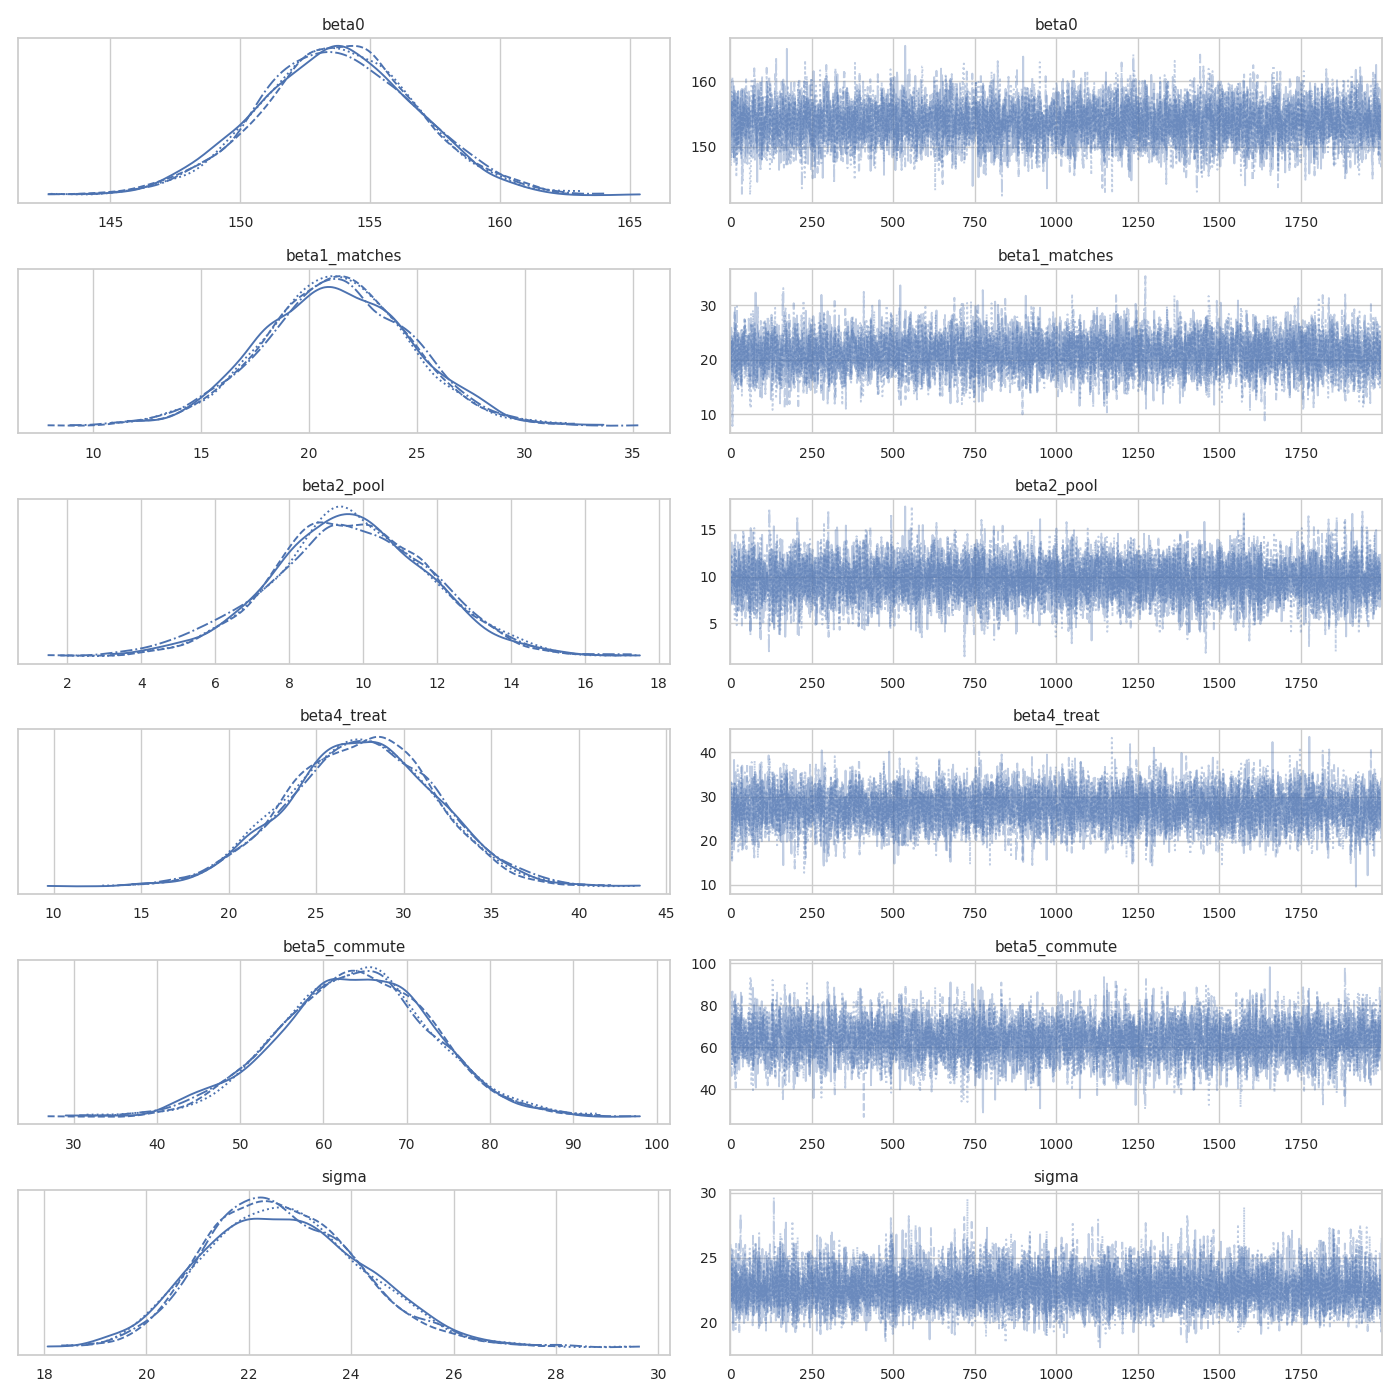
\includegraphics[width=0.8\textwidth]{resultados_rider_cancellation/05_traceplot.png}
    \caption{Distribuciones Posteriores (Traceplot): Evaluación de la estabilidad para el modelo de cancelaciones.}
    \label{fig:uber_trace}
\end{figure}

Para interpretar este gráfico no necesitas saber cálculos complejos, solo observar dos aspectos visuales del comportamiento algorítmico:
\begin{itemize}
    \item \textbf{El panel izquierdo:} Si las diferentes líneas de colores logran formar juntas curvas redondeadas y suaves como "campanitas", significa que el proceso sí logró hallar el centro en el que se ubica la verdad. 
    \item \textbf{El panel derecho:} Para un estadístico esta es la parte clave. Si allí todo parece una mancha ruidosa e irregular como si fuera una "oruga peluda" (así se le apoda en la industria), entonces es una gran noticia. Significa que el computador barajó y exploró de manera muy eficiente miles de valores sin quedarse trabado en ninguno matemático en especial. Aprobamos este chequeo.
\end{itemize}

\subsubsection*{2. Respondiendo a la pregunta principal (Forest Plot e Intervalo HDI)}

Resueltos los aspectos aburridos y de estabilidad interna, podemos por fin buscar la respuesta principal del proyecto: \textit{¿Afecta negativamente hacer que un pasajero espere 5 minutos intentando buscar su Uber Pool, o da matemáticamente igual y podíamos ahorrar gastos operativos?}

A diferencia de la estadística de colegio elemental que dictamina que todo es un único resultado irrefutable; nosotros usamos Inferencia Bayesiana donde impera un concepto bellísimo llamado \textbf{HDI al 95\%} (Intervalo de Alta Densidad).
Para entenderlo simple, un HDI es como decirle a tu jefe: \textit{"No pondré mis manos al fuego lanzándote el número exacto del impacto de este cambio, pero estoy 95\% seguro de que, tome el número que tome, vivirá dentro de este rango que va desde el número A hasta el número B"}. 

Veamos de forma visual cuáles fueron los HDI de nuestro problema:
\begin{figure}[H]
    \centering
    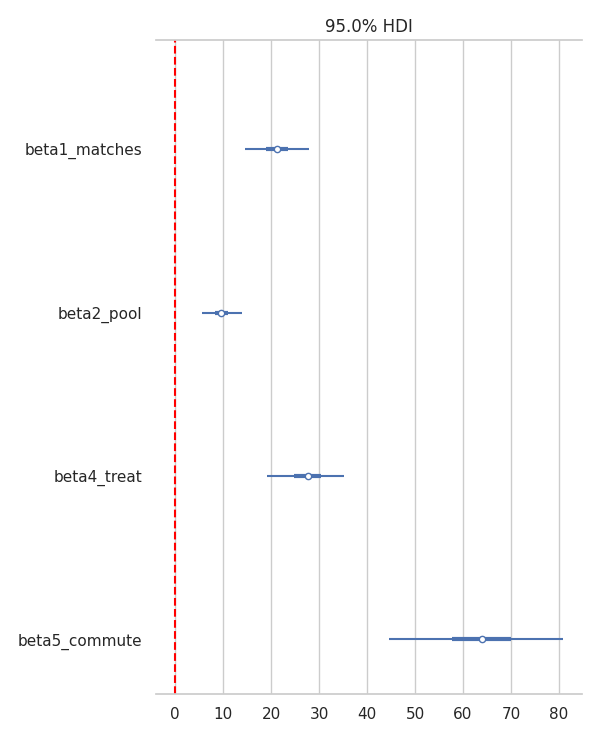
\includegraphics[width=0.7\textwidth]{resultados_rider_cancellation/09_forest_plot.png}
    \caption{Intervalos de Credibilidad del 95\% (Forest Plot): Impacto real en las cancelaciones.}
    \label{fig:uber_forest}
\end{figure}

Al leer los "bigotes azules" de este gráfico, obtenemos una conclusión radicalmente distinta a la del volumen de viajes:
\begin{itemize}
    \item \textbf{Efecto del Tratamiento (\textit{beta\_treat}):} El intervalo HDI al 95\% se ubica entre \textbf{[18.9 y 35.7]} cancelaciones adicionales. Lo más importante: \textbf{el intervalo NO cruza el cero}. Esto indica una evidencia estadística sólida de que aumentar la espera a 5 minutos incrementa sistemáticamente las cancelaciones.
    \item \textbf{Efecto de Hora Pico (\textit{beta\_commute}):} Con un rango de \textbf{[47.0 a 83.0]}, confirmamos que la congestión urbana es el mayor disparador de frustración del usuario en Bogotá.
\end{itemize}

\subsubsection*{3. Prueba final: ¿El modelo logra parecerse a Uber? (Gráfica PPC)}

Por muy impresionante que haya sido la estadística, antes de decirle algo oficial a la plana directiva solicitamos que se genere una prueba de fuego, el Chequeo Predictivo de Ajustes o \textbf{PPC}. Este le pide a la computadora que ya "conoce" la receta inventarse una tarde de viajes nueva y la compare junto a los datos crudos de las verdaderas tardes brindadas por Uber.

\begin{figure}[H]
    \centering
    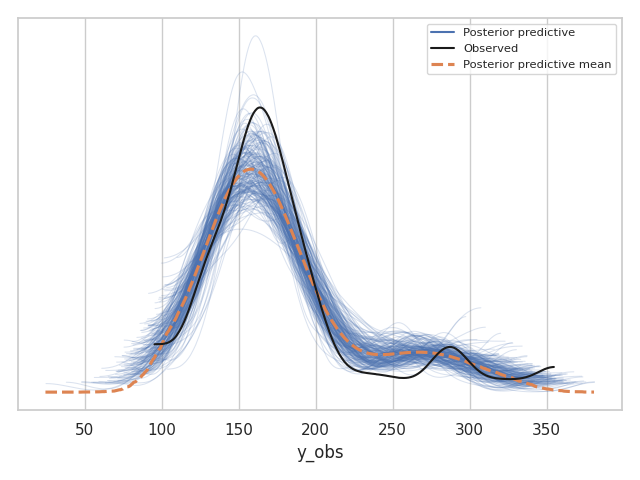
\includegraphics[width=0.65\textwidth]{resultados_rider_cancellation/10_ppc.png}
    \caption{PPC: Validación predictiva para el modelo de fricción del usuario.}
    \label{fig:uber_ppc}
\end{figure}
La gráfica contesta nuestras dudas de forma elocuente. Como queda claro, tanto las múltiples iteraciones azules de la máquina como la media del modelo logran capturar la estructura de los datos reales de cancelaciones.

\subsubsection*{Conclusión Operativa: La Radiografía de la Impaciencia}

¿Qué significa esto para Uber Bogotá? A diferencia del análisis simple de volumen de viajes, el modelo de cancelaciones revela que **el usuario bogotano sí penaliza la espera**. 

El hecho de que el intervalo de \textit{beta\_treat} no cruce el cero es una señal de alerta para el área logística. Si bien obligar al usuario a esperar 5 minutos puede parecer una "eficiencia" en el papel, en la práctica estamos empujando a ~28 usuarios adicionales por periodo a cancelar su viaje. Esto no es solo pérdida de ingresos inmediata, sino un daño potencial a la lealtad de marca a largo plazo. 

En conclusión, la demanda de Uber Pool en Bogotá demuestra ser **elástica frente a la frustración**. Los resultados sugieren que cualquier política de "espera intencional" debe ser compensada con estrategias de incentivos o, mejor aún, con un despliegue predictivo de flota basado en los patrones que analizaremos en la siguiente fase del taller (Multinomial).

\end{document}
